%%%%%%%%%%%%%%%%%%%%%%%%%%%%%%%%%%%%%%%%%%%%%%%%%%%%%%%%%%%%%%%%%%%%%%%%%%%%%%%%
% Enclosure & Controls
%%%%%%%%%%%%%%%%%%%%%%%%%%%%%%%%%%%%%%%%%%%%%%%%%%%%%%%%%%%%%%%%%%%%%%%%%%%%%%%%
\part{Enclosure \& Controls} \label{Enclosure}

%%%%%%%%%%%%%%%%%%%%%%%%%%%%%%%%%%%%%%%%%%%%%%%%%%%%%%%%%%%%%%%%%%%%%%%%%%%%%%%%
% Introduction
%%%%%%%%%%%%%%%%%%%%%%%%%%%%%%%%%%%%%%%%%%%%%%%%%%%%%%%%%%%%%%%%%%%%%%%%%%%%%%%%
\chapter{Introduction}

The enclosure is made of \wood{} wood with a dewaxed shellac finish. The front
panel is made of \front{}.

\par\bigskip

\danger{Do not get alcohol anywhere near this.  The wood finish is shellac
whose solvent is alcohol.  Alcohol will ruin the finish, i.e. dissolve it like
turpentine will with oil based paint.  So don't rest your beer bottle, glass of
wine or shot of tequila on top.  And to be safe, don't clean it with any kind of
chemical cleaning solution.  A dry or slightly damp rag, preferably microfiber,
should be sufficient to get fingerprints, dust and other crud off of the wood
finish and \front{} front - see the \hyperref[Cleaning]{Cleaning} section.}

\par\bigskip

\danger{Before trying to disassemble the enclosure to either replace the
\hyperref[Coin Cell Battery]{\cCC{f}} or remove the
\hyperref[Micro SD Card]{\cMSD{f}} card, please read the
\hyperref[Disassembly]{Disassembly} section.}

%%%%%%%%%%%%%%%%%%%%%%%%%%%%%%%%%%%%%%%%%%%%%%%%%%%%%%%%%%%%%%%%%%%%%%%%%%%%%%%%
% Front
%%%%%%%%%%%%%%%%%%%%%%%%%%%%%%%%%%%%%%%%%%%%%%%%%%%%%%%%%%%%%%%%%%%%%%%%%%%%%%%%
\chapter{Front} \label{Front}

The \cFr{f} is made of \front{} with cast acrylic windows for the
\hyperref[Display]{\cDi{f}} and \hyperref[Lighting]{\cLi{f}}. It contains all of
the controls and screens necessary for interacting with the device except for
the \hyperref[Touch Sensor]{\cTS{f}} which is located underneath the
\hyperref[Top]{\cTo{f}} of the enclosure.

\begin{figure}[H]
\centering
  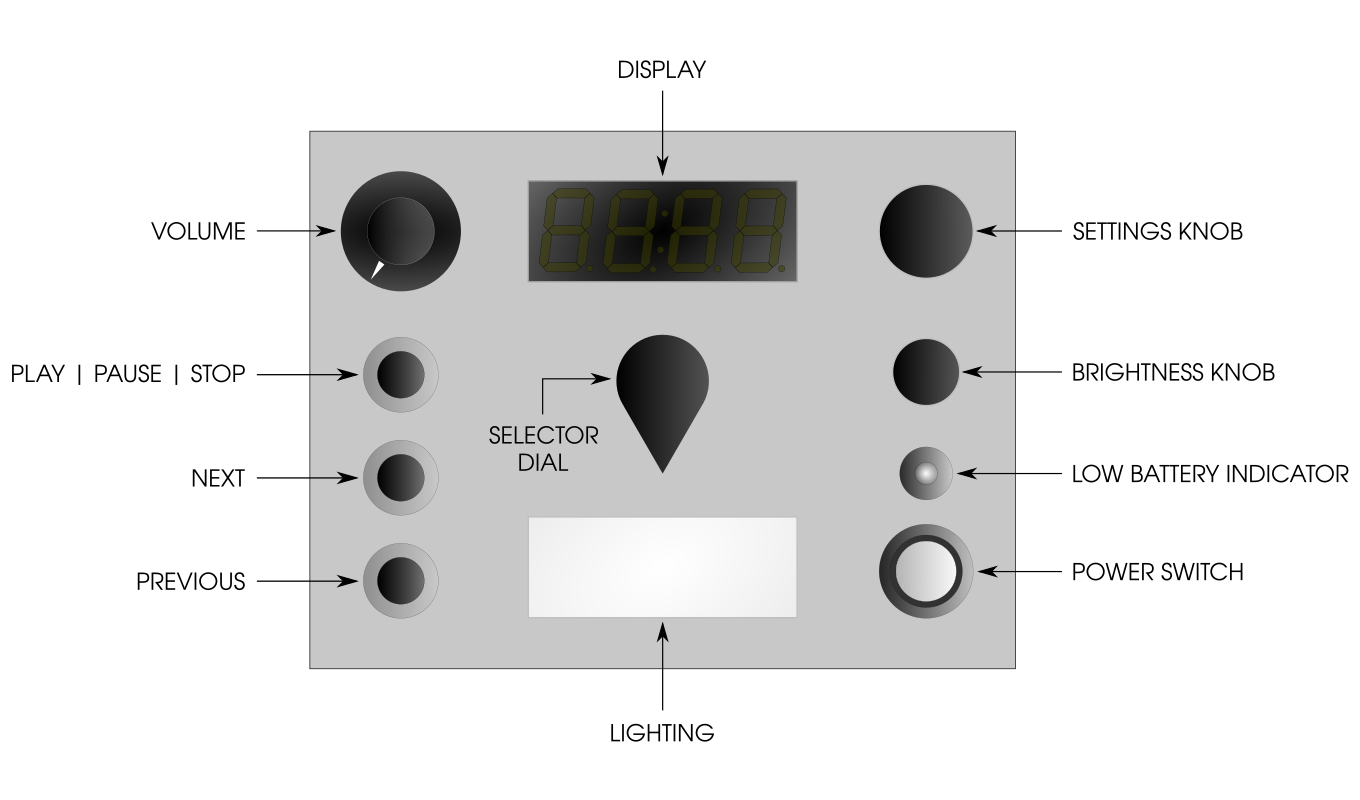
\includegraphics{images/front_panel.png}
\caption{Front}
\end{figure}

%%%%%%%%%%%%%%%%%%%%%%%%%%%%%%%%%%%%%%%%%%%%%%%%%%%%%%%%%%%%%%%%%%%%%%%%%%%%%%%%
% Front - Power
%%%%%%%%%%%%%%%%%%%%%%%%%%%%%%%%%%%%%%%%%%%%%%%%%%%%%%%%%%%%%%%%%%%%%%%%%%%%%%%%
\section{Power}

%%%%%%%%%%%%%%%%%%%%%%%%%%%%%%%%%%%%%%%%%%%%%%%%%%%%%%%%%%%%%%%%%%%%%%%%%%%%%%%%
% Front - Power - Power Switch
%%%%%%%%%%%%%%%%%%%%%%%%%%%%%%%%%%%%%%%%%%%%%%%%%%%%%%%%%%%%%%%%%%%%%%%%%%%%%%%%
\subsection{Power Switch} \label{Power Switch}

The \cPo{f} is a latching switch used to turn the device \sON{f} and \sOFF{f}.
\begin{itemize}
  \item To turn the device \sON{f}, press inward until you hear a mechanical
    click and feel it lock in place.
  \item To turn the device \sOFF{f}, press inward until you hear a mechanical
    click and feel it release.
\end{itemize}

You can visually tell whether the switch is \sON{f} or \sOFF{f} by whether or
not it is lit.\footnote{ The color of the light may vary.}

\begin{table}[H]
\ers{1}
\centering
\begin{tabu} to 7cm { X[1,c,m] X[1,c,m] }
  \sON{n} & \sOFF{n} \\
  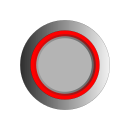
\includegraphics{images/onoff_on.png} & 
\includegraphics{images/onoff_off.png} \\
\end{tabu}
\caption{Power Switch - ON | OFF Indication}
\end{table}

It will also be flush with the bevel when \sOFF{f} and sunken in when \sON{f}.

\par\medskip

A few items of note:

\begin{itemize}
  \item When the device is plugged in there is no need to switch the device
    \sOFF{f}.
  \item To reduce power consumption when running unplugged, instead of switching
    the device \sOFF{f}, you can:
    \begin{itemize}
      \item Use the \hyperref[Brightness Knob]{\cBr{f}} to blank both the
        \hyperref[Display]{\cDi{f}} and \hyperref[Lighting]{\cLi{f}}.
      \item Use the \hyperref[Play|Pause|Stop]{\cPl{f}} push-button to \sAuSt{f}
        the \hyperref[Audio]{\mAu{f}}.
      \item Set \mPSNa{f}, \mPSSt{f} and/or \mPSSl{f} timers or forcibly put the
        device to sleep using \mPSTo{f} - see \hyperref[Power Settings]{\mPS{f}}
        for configuration and usage.
    \end{itemize}
\end{itemize}

%%%%%%%%%%%%%%%%%%%%%%%%%%%%%%%%%%%%%%%%%%%%%%%%%%%%%%%%%%%%%%%%%%%%%%%%%%%%%%%%
% Front - Power - Low Battery Indicator
%%%%%%%%%%%%%%%%%%%%%%%%%%%%%%%%%%%%%%%%%%%%%%%%%%%%%%%%%%%%%%%%%%%%%%%%%%%%%%%%
\subsection{Low Battery Indicator} \label{Low Battery Indicator}

The \cLB{f} is a red LED and is used to indicate that the device needs to be
recharged.  When the light turns on, the battery charge is getting low.

\begin{table}[H]
\ers{1}
\centering
\begin{tabu} to 6cm { X[1,c,m] X[1,c,m] }
  OK & LOW \\
  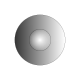
\includegraphics{images/lowbat_off.png}
    & 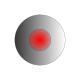
\includegraphics{images/lowbat_on.png} \\
\end{tabu}
\caption{Low Battery Indicator}
\end{table}

Note that when music is playing, the light might flicker on and off. This is
because the electric current varies a great deal when playing audio and a high
volume setting and/or certain sounds (usually low end sounds) can cause the
voltage in the circuit to temporarily drop triggering the \cLB{f}.  Turning
the volume down may get rid of the flicker.  Either way, the battery should
be recharged.

%%%%%%%%%%%%%%%%%%%%%%%%%%%%%%%%%%%%%%%%%%%%%%%%%%%%%%%%%%%%%%%%%%%%%%%%%%%%%%%%
% Front - Screens
%%%%%%%%%%%%%%%%%%%%%%%%%%%%%%%%%%%%%%%%%%%%%%%%%%%%%%%%%%%%%%%%%%%%%%%%%%%%%%%%
\section{Screens}

%%%%%%%%%%%%%%%%%%%%%%%%%%%%%%%%%%%%%%%%%%%%%%%%%%%%%%%%%%%%%%%%%%%%%%%%%%%%%%%%
% Front - Screens - Display
%%%%%%%%%%%%%%%%%%%%%%%%%%%%%%%%%%%%%%%%%%%%%%%%%%%%%%%%%%%%%%%%%%%%%%%%%%%%%%%%
\subsection{Display} \label{Display}

The \cDi{f} is the primary means of conveying information.  It is an LED
\href{https://en.wikipedia.org/wiki/Seven-segment\_display}{Seven-Segment Display}
and can display the full range of numerical digits as well as the majority of
letters.\footnote{ See \hyperref[Display Digits]{Number \& Letter Display Representations}
in the Appendix for a complete list.}  It can also display a decimal point after
each digit and a colon in the middle.

\par\medskip

The brightness of the \cDi{f} is controlled by the
\hyperref[Brightness Knob]{\cBr{f}}.

%%%%%%%%%%%%%%%%%%%%%%%%%%%%%%%%%%%%%%%%%%%%%%%%%%%%%%%%%%%%%%%%%%%%%%%%%%%%%%%%
% Front - Screens - Lighting
%%%%%%%%%%%%%%%%%%%%%%%%%%%%%%%%%%%%%%%%%%%%%%%%%%%%%%%%%%%%%%%%%%%%%%%%%%%%%%%%
\subsection{Lighting} \label{Lighting}

The \cLi{f} is made up of \num{16} RGB LEDs - 2 rows with \num{8} in each row.
A translucent white plastic called Delrin is used to diffuse the light.  Its
primary use is as a night light or timer status indicator.
See \hyperref[Clock]{\mCl{f}} and \hyperref[Timer]{\mTi{f}} respectively for
more information on its use and \hyperref[Set Night Light]{\mSN{f}} for
instructions on setting the \num{3} configurable night light colors.

\par\medskip

The brightness of the \cLi{f} window is controlled by the
\hyperref[Brightness Knob]{\cBr{f}}.

%%%%%%%%%%%%%%%%%%%%%%%%%%%%%%%%%%%%%%%%%%%%%%%%%%%%%%%%%%%%%%%%%%%%%%%%%%%%%%%%
% Front - Screens - Brightness Knob
%%%%%%%%%%%%%%%%%%%%%%%%%%%%%%%%%%%%%%%%%%%%%%%%%%%%%%%%%%%%%%%%%%%%%%%%%%%%%%%%
\subsection{Brightness Knob} \label{Brightness Knob}

The \cBr{f} is an optical rotary encoder and is used to control the brightness
of both the \hyperref[Display]{\cDi{f}} and \hyperref[Lighting]{\cLi{f}}. It
does not have start or stop positions and will turn indefinitely in either
direction.

\begin{itemize}
  \item Turn \textit{clockwise} to \textit{increase} the brightness.
  \item Turn \textit{counter-clockwise} to \textit{decrease} the
    brightness.\footnote{ The \cDi{ss} does not dim seamlessly and you will
    likely notice that it jumps or drops in brightness.  This is normal
    behavior as the hardware only supports \num{16} brightness levels.}
\end{itemize}

Continually turning in one direction or the other will eventually either:

\begin{enumerate}
  \item Reach a \textit{maximum} brightness, or
  \item Blank both the \cDi{f} and \cLi{f}.
\end{enumerate}

\info{When running on battery power and not using the \cDi{f} or \cLi{f} - for
example, if just listening to music - turn the \cBr{f} \textit{counter-clockwise}
until they go blank to prolong battery charge.}

%%%%%%%%%%%%%%%%%%%%%%%%%%%%%%%%%%%%%%%%%%%%%%%%%%%%%%%%%%%%%%%%%%%%%%%%%%%%%%%%
% Front - UI Controls
%%%%%%%%%%%%%%%%%%%%%%%%%%%%%%%%%%%%%%%%%%%%%%%%%%%%%%%%%%%%%%%%%%%%%%%%%%%%%%%%
\section{UI Controls}

The \cRs{f} and \cEs{f} are the primary controls used to interact with the
device and make use of its functionality.

%%%%%%%%%%%%%%%%%%%%%%%%%%%%%%%%%%%%%%%%%%%%%%%%%%%%%%%%%%%%%%%%%%%%%%%%%%%%%%%%
% Front - UI Controls - Selector Dial
%%%%%%%%%%%%%%%%%%%%%%%%%%%%%%%%%%%%%%%%%%%%%%%%%%%%%%%%%%%%%%%%%%%%%%%%%%%%%%%%
\subsection{Selector Dial} \label{Selector Dial}

The \cRs{f} is a \num{3} position, \num{90}° angle rotary switch and is
used to select available operational modes.

\begin{table}[H]
\ers{0.1}
\centering
\begin{tabu}{ c c c }
  \dLe{f} & \dMi{f} & \dRi{f} \\
  \sLe & \sMi & \sRi
\end{tabu}
\caption{Selector Dial Positions}
\end{table}

For information on usage, see \hyperref[Operation - Selector Dial]{\cRs{f}} in
the \hyperref[Operation]{Operation} chapter.

%%%%%%%%%%%%%%%%%%%%%%%%%%%%%%%%%%%%%%%%%%%%%%%%%%%%%%%%%%%%%%%%%%%%%%%%%%%%%%%%
% Front - UI Controls - Settings Knob
%%%%%%%%%%%%%%%%%%%%%%%%%%%%%%%%%%%%%%%%%%%%%%%%%%%%%%%%%%%%%%%%%%%%%%%%%%%%%%%%
\subsection{Settings Knob} \label{Settings Knob}

The \cEs{f} is a combination optical rotary encoder w/ detents \textit{and}
momentary switch which can be both \textit{turned} and \textit{pressed}.  It
does \textit{not} have start or stop positions and will turn indefinitely in
either direction.

\par\medskip

For information on usage, see \hyperref[Operation - Settings Knob]{\cEs{f}} in
the \hyperref[Operation]{Operation} chapter.

%%%%%%%%%%%%%%%%%%%%%%%%%%%%%%%%%%%%%%%%%%%%%%%%%%%%%%%%%%%%%%%%%%%%%%%%%%%%%%%%
% Front - Audio Controls
%%%%%%%%%%%%%%%%%%%%%%%%%%%%%%%%%%%%%%%%%%%%%%%%%%%%%%%%%%%%%%%%%%%%%%%%%%%%%%%%
\section{Audio Controls}

The left side of the front panel is devoted to the \hyperref[Audio]{\mAu{f}}.

%%%%%%%%%%%%%%%%%%%%%%%%%%%%%%%%%%%%%%%%%%%%%%%%%%%%%%%%%%%%%%%%%%%%%%%%%%%%%%%%
% Front - Audio Controls - Volume
%%%%%%%%%%%%%%%%%%%%%%%%%%%%%%%%%%%%%%%%%%%%%%%%%%%%%%%%%%%%%%%%%%%%%%%%%%%%%%%%
\subsection{Volume} \label{Volume}

The \cVo{f} knob is a dual-gang potentiometer and controls the volume level of
the \mAu{f}\footnote{ The \cVo{ss} knob is not connected to the \cBe{ss} so
cannot control its volume.} and has a \textit{white arrow} indicator on the
sleeve.  Unlike the \hyperref[Settings Knob]{\cEs{f}} and
\hyperref[Brightness Knob]{\cBr{f}} it does \textit{not} turn indefinitely and
has physical start and stop positions.

\par\medskip

For usage information, see \hyperref[Audio - Volume]{\cVo{f}} in the
\hyperref[Audio]{\mAu{f}} section.

%%%%%%%%%%%%%%%%%%%%%%%%%%%%%%%%%%%%%%%%%%%%%%%%%%%%%%%%%%%%%%%%%%%%%%%%%%%%%%%%
% Front - Audio Controls - Play|Pause|Stop
%%%%%%%%%%%%%%%%%%%%%%%%%%%%%%%%%%%%%%%%%%%%%%%%%%%%%%%%%%%%%%%%%%%%%%%%%%%%%%%%
\subsection{Play | Pause | Stop} \label{Play|Pause|Stop}

\cPl{f} is a momentary push-button and is used to \sAuPl{f}, \sAuPa{f} and
\sAuSt{f} the \mAu{f}.

\par\medskip

For usage information, see \hyperref[Audio - Play|Pause|Stop]{\cPl{f}} in the
\hyperref[Audio]{\mAu{f}} section.

%%%%%%%%%%%%%%%%%%%%%%%%%%%%%%%%%%%%%%%%%%%%%%%%%%%%%%%%%%%%%%%%%%%%%%%%%%%%%%%%
% Front - Audio Controls - Next
%%%%%%%%%%%%%%%%%%%%%%%%%%%%%%%%%%%%%%%%%%%%%%%%%%%%%%%%%%%%%%%%%%%%%%%%%%%%%%%%
\subsection{Next} \label{Next}

\cNe{f} is a momentary push-button and is used to \sAuSk{f} \textit{forward} one
or more tracks.

\par\medskip

For usage information, see \hyperref[Audio - Next]{\cNe{f}} in the
\hyperref[Audio]{\mAu{f}} section.

%%%%%%%%%%%%%%%%%%%%%%%%%%%%%%%%%%%%%%%%%%%%%%%%%%%%%%%%%%%%%%%%%%%%%%%%%%%%%%%%
% Front - Audio Controls - Previous
%%%%%%%%%%%%%%%%%%%%%%%%%%%%%%%%%%%%%%%%%%%%%%%%%%%%%%%%%%%%%%%%%%%%%%%%%%%%%%%%
\subsection{Previous} \label{Previous}

\cPr{f} is a momentary push-button and is used to \sAuSk{f} \textit{backward}
one or more tracks or \textit{rewind} the current track.

\par\medskip

For usage information, see \hyperref[Audio - Previous]{\cPr{f}} in the
\hyperref[Audio]{\mAu{f}} section.

%%%%%%%%%%%%%%%%%%%%%%%%%%%%%%%%%%%%%%%%%%%%%%%%%%%%%%%%%%%%%%%%%%%%%%%%%%%%%%%%
% Top
%%%%%%%%%%%%%%%%%%%%%%%%%%%%%%%%%%%%%%%%%%%%%%%%%%%%%%%%%%%%%%%%%%%%%%%%%%%%%%%%
\chapter{Top} \label{Top}

Attached to the underside of the \cTo{f} is a \cTS{f} and a \cCC{f} and holder.

\begin{figure}[H]
\centering
  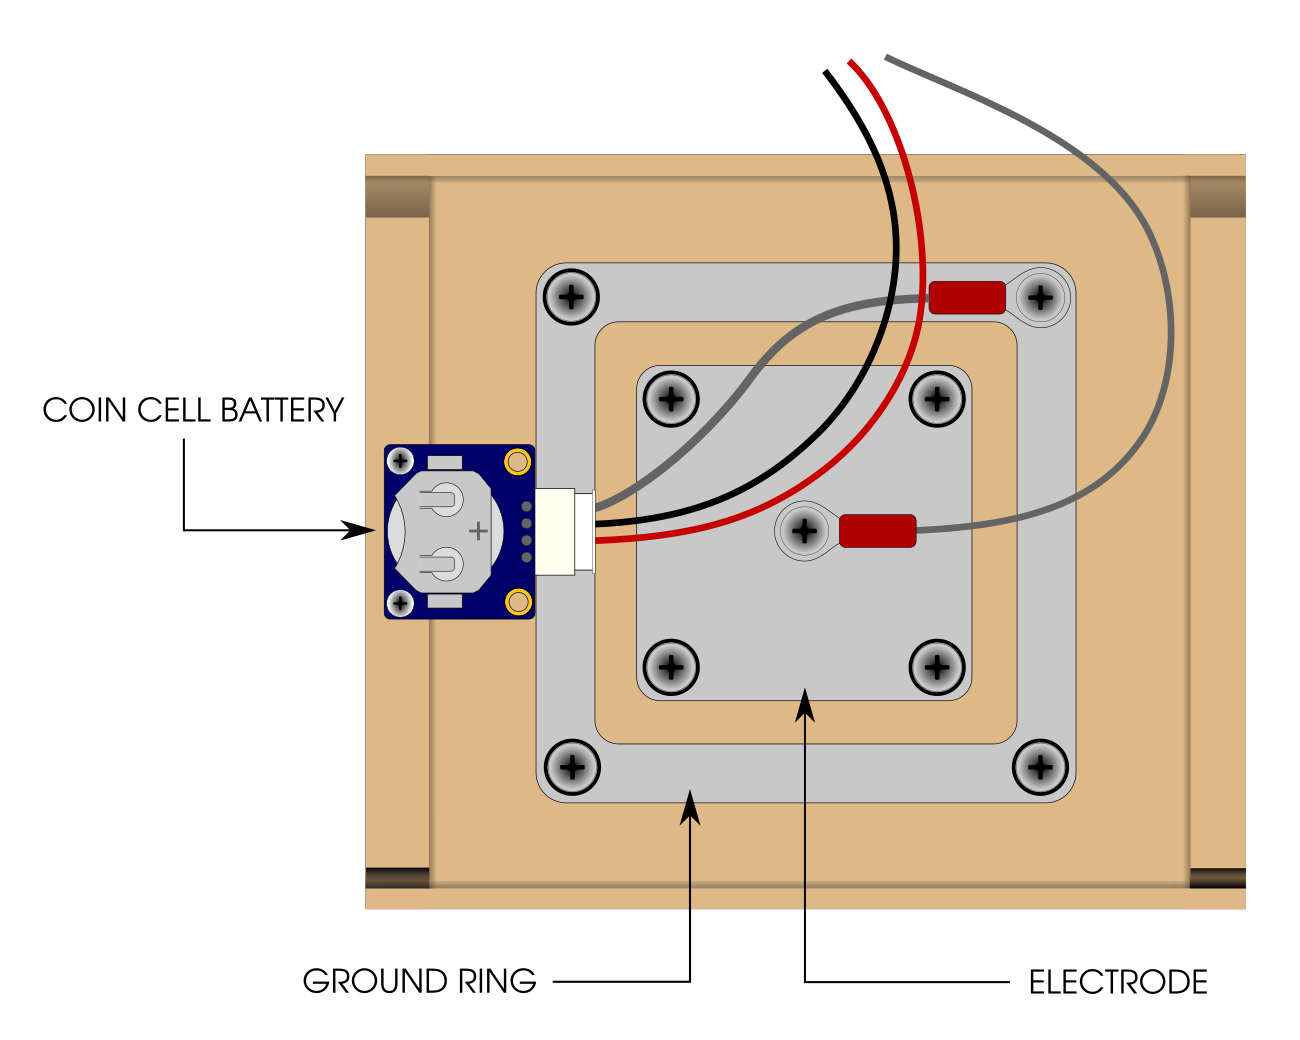
\includegraphics{images/top.png}
\caption{Top}
\end{figure}

%%%%%%%%%%%%%%%%%%%%%%%%%%%%%%%%%%%%%%%%%%%%%%%%%%%%%%%%%%%%%%%%%%%%%%%%%%%%%%%%
% Top - Touch Sensor
%%%%%%%%%%%%%%%%%%%%%%%%%%%%%%%%%%%%%%%%%%%%%%%%%%%%%%%%%%%%%%%%%%%%%%%%%%%%%%%%
\section{Touch Sensor} \label{Touch Sensor}

The \cTS{f}, also called an \textit{electrode}, is made of a \num{2$\times$2}
inch square of \mono{1/32"} thick aluminum with a wire running to the
microcontroller.  Around the electrode is an aluminum ground ring.

\par\medskip

For more information, see \hyperref[Operation - Touch Sensor]{\cTS{f}} in the
\hyperref[Operation]{Operation} chapter and \hyperref[Touch Settings]{\mTS{f}}
for how to enable and configure the touch capability of the device.

%%%%%%%%%%%%%%%%%%%%%%%%%%%%%%%%%%%%%%%%%%%%%%%%%%%%%%%%%%%%%%%%%%%%%%%%%%%%%%%%
% Top - Coin Cell Battery
%%%%%%%%%%%%%%%%%%%%%%%%%%%%%%%%%%%%%%%%%%%%%%%%%%%%%%%%%%%%%%%%%%%%%%%%%%%%%%%%
\section{Coin Cell Battery} \label{Coin Cell Battery}

The \cCC{f} is a \mono{3\thinspace V} \mono{CR2032} Lithium battery and is used
to keep the date and time updated when the device is switched \sOFF{f} via the
\hyperref[Power Switch]{\cPo{f}} and otherwise unpowered.  It is attached on the
left side just underneath the \cTo{f}.  It is \textit{not} rechargeable,
however, it should last for a number of years before needing replacement.  You
will know it needs replacing if the date and time are not correct when switching
the device \sON{f} (assuming they were correct before switching the device
\sOFF{f}).  For more information see
\hyperref[Replacing Battery]{Replacing the Coin Cell Battery}.

%%%%%%%%%%%%%%%%%%%%%%%%%%%%%%%%%%%%%%%%%%%%%%%%%%%%%%%%%%%%%%%%%%%%%%%%%%%%%%%%
% Bottom
%%%%%%%%%%%%%%%%%%%%%%%%%%%%%%%%%%%%%%%%%%%%%%%%%%%%%%%%%%%%%%%%%%%%%%%%%%%%%%%%
\chapter{Bottom} \label{Bottom}

The \cBo{f} holds and secures the \cRB{f}.

\begin{figure}[H]
\centering
  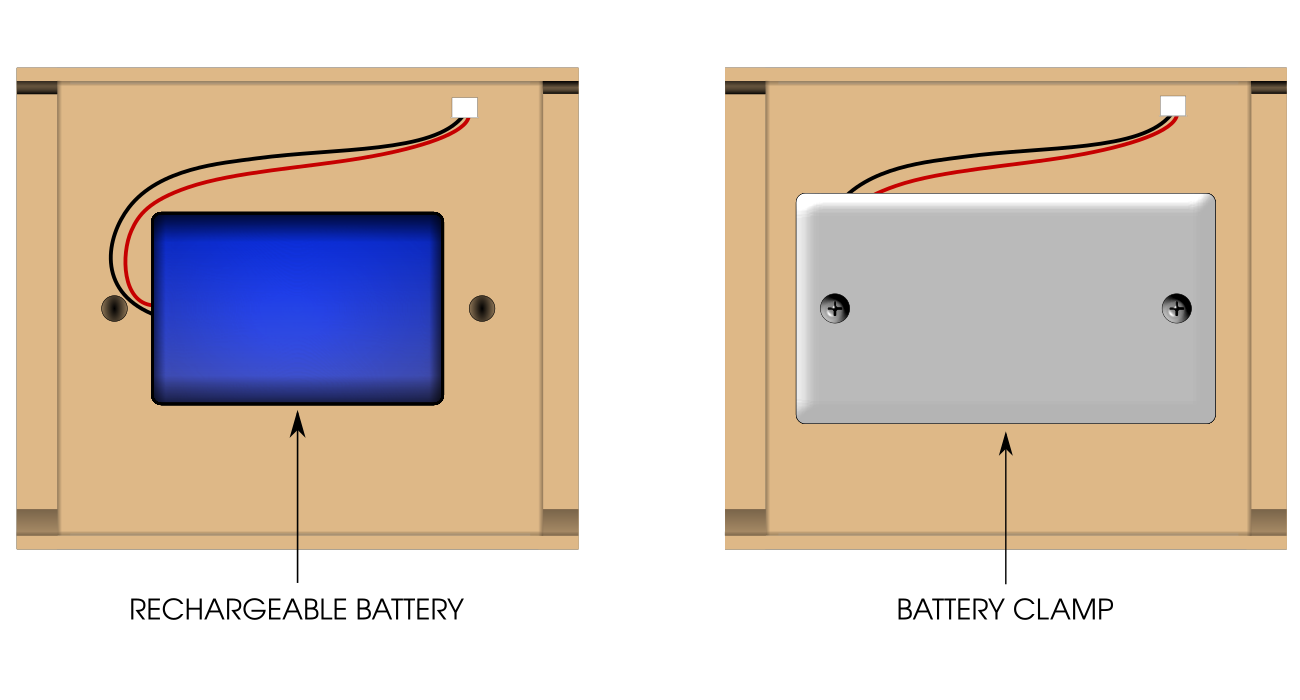
\includegraphics{images/bottom.png}
\caption{Bottom}
\end{figure}

%%%%%%%%%%%%%%%%%%%%%%%%%%%%%%%%%%%%%%%%%%%%%%%%%%%%%%%%%%%%%%%%%%%%%%%%%%%%%%%%
% Bottom - Rechargeable Battery
%%%%%%%%%%%%%%%%%%%%%%%%%%%%%%%%%%%%%%%%%%%%%%%%%%%%%%%%%%%%%%%%%%%%%%%%%%%%%%%%
\section{Rechargeable Battery} \label{Rechargeable Battery}

The \cRB{f} is a nominal \mono{3.7\thinspace V}, \mono{6600\thinspace mAh}
Lithium Ion battery pack.  It is the primary power source when the device is
unplugged and switched \sON{f}.  With music playing, the charge should last
about a day.

%%%%%%%%%%%%%%%%%%%%%%%%%%%%%%%%%%%%%%%%%%%%%%%%%%%%%%%%%%%%%%%%%%%%%%%%%%%%%%%%
% Sides
%%%%%%%%%%%%%%%%%%%%%%%%%%%%%%%%%%%%%%%%%%%%%%%%%%%%%%%%%%%%%%%%%%%%%%%%%%%%%%%%
\chapter{Sides} \label{Sides}

The \cSi{f} house the speakers and are where the screws that secure the
enclosure are.

\begin{figure}[H]
\centering
  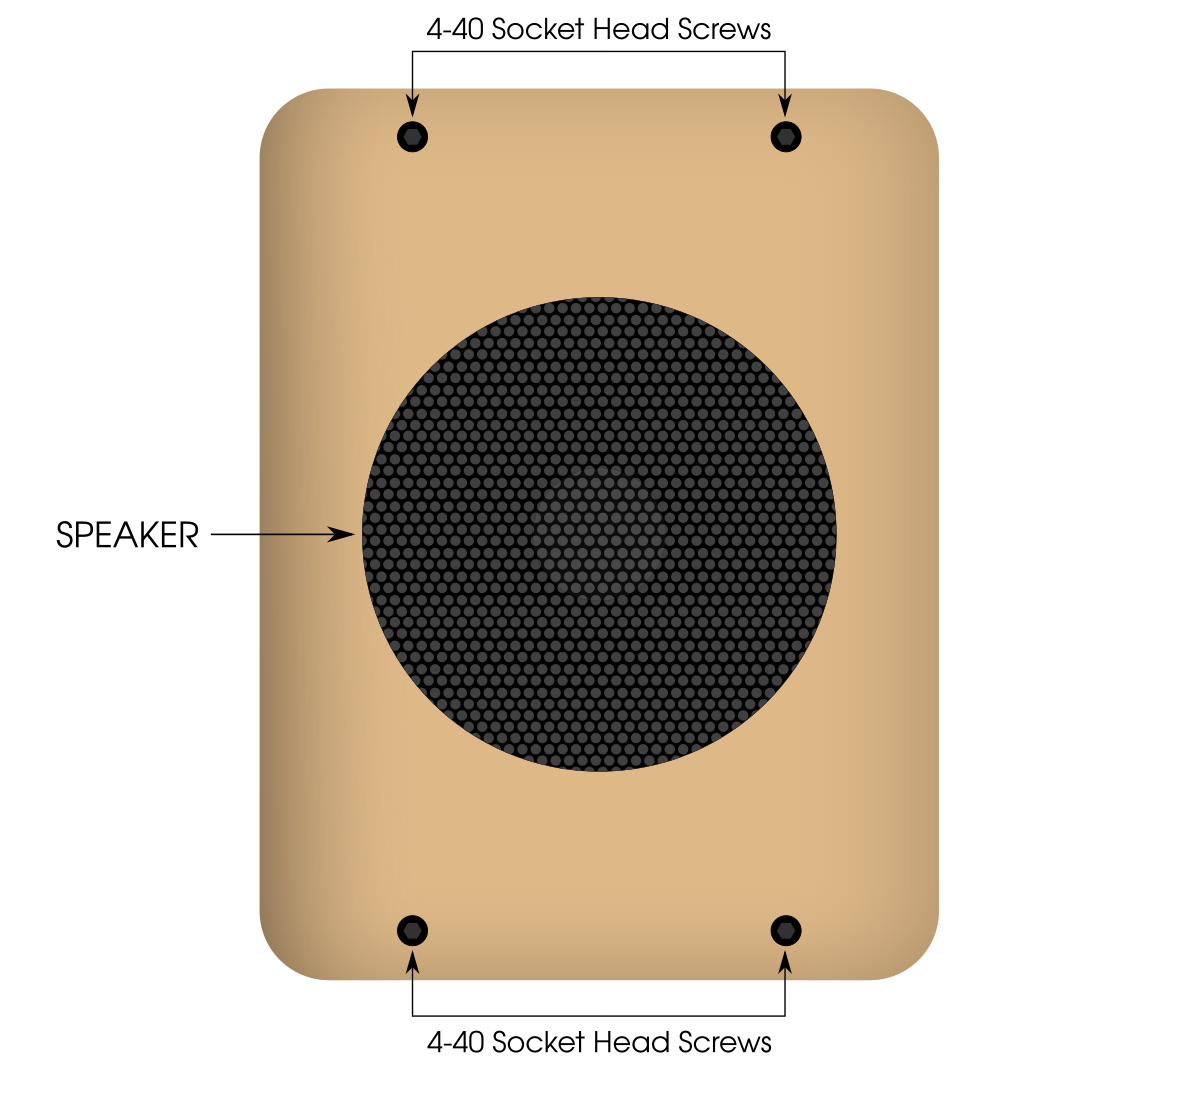
\includegraphics{images/side.png}
\caption{Side}
\end{figure}

%%%%%%%%%%%%%%%%%%%%%%%%%%%%%%%%%%%%%%%%%%%%%%%%%%%%%%%%%%%%%%%%%%%%%%%%%%%%%%%%
% Sides - Speakers
%%%%%%%%%%%%%%%%%%%%%%%%%%%%%%%%%%%%%%%%%%%%%%%%%%%%%%%%%%%%%%%%%%%%%%%%%%%%%%%%
\section{Speakers} \label{Speakers}

The \num{2} speakers, one on each side, are \mono{8\thinspace\small{$\Omega$}},
\mono{2\thinspace W}, \mono{99\thinspace dB} with paper cone and ferrite magnet.
They are used in conjunction with the \hyperref[Audio]{\mAu{f}}.  The grills are
made of \mono{1/32"} inch, \num{24} gauge perforated \num{304} stainless steel,
painted black.

%%%%%%%%%%%%%%%%%%%%%%%%%%%%%%%%%%%%%%%%%%%%%%%%%%%%%%%%%%%%%%%%%%%%%%%%%%%%%%%%
% Sides - Fastening Screws
%%%%%%%%%%%%%%%%%%%%%%%%%%%%%%%%%%%%%%%%%%%%%%%%%%%%%%%%%%%%%%%%%%%%%%%%%%%%%%%%
\section{Fastening Screws} \label{Fastening Screws}

The screws used to keep the enclosure together are \mono{4-40} Socket Head
screws made of Black-Oxide Alloy Steel and have a \mono{3/32"} hex wrench drive
size.  There are a total of \num{8} screws with \num{4} on each side.

\warning{Before taking the enclosure apart, please refer to
\hyperref[Disassembly]{Disassembly}.}

A \mono{3/32"} \hyperref[Hex Driver]{Hex Driver} is included for the purpose
of removing and replacing these screws.  The use of a straight driver as
opposed to a bent key is recommended in order to lessen the possibility of
scraping the finish on the wood.

%%%%%%%%%%%%%%%%%%%%%%%%%%%%%%%%%%%%%%%%%%%%%%%%%%%%%%%%%%%%%%%%%%%%%%%%%%%%%%%%
% Back
%%%%%%%%%%%%%%%%%%%%%%%%%%%%%%%%%%%%%%%%%%%%%%%%%%%%%%%%%%%%%%%%%%%%%%%%%%%%%%%%
\chapter{Back} \label{Back}

On the \cBa{f} of the device is the \cPP{f} that is used to both power the
device and charge the \hyperref[Rechargeable Battery]{\cRB{f}} inside.

\begin{figure}[H]
\centering
  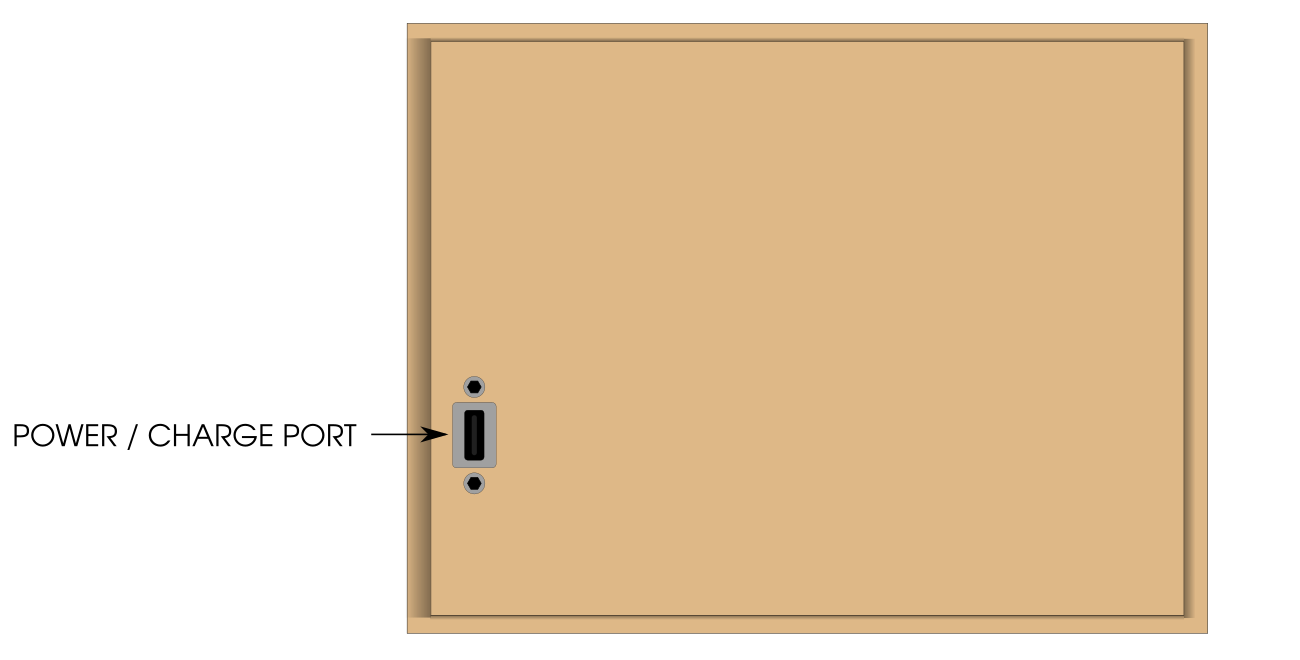
\includegraphics{images/back.png}
\caption{Back}
\end{figure}

The main circuit board is attached on the inside.  Of interest are
the \cBe{f} and removable \cMSD{f}.

\begin{figure}[H]
\centering
  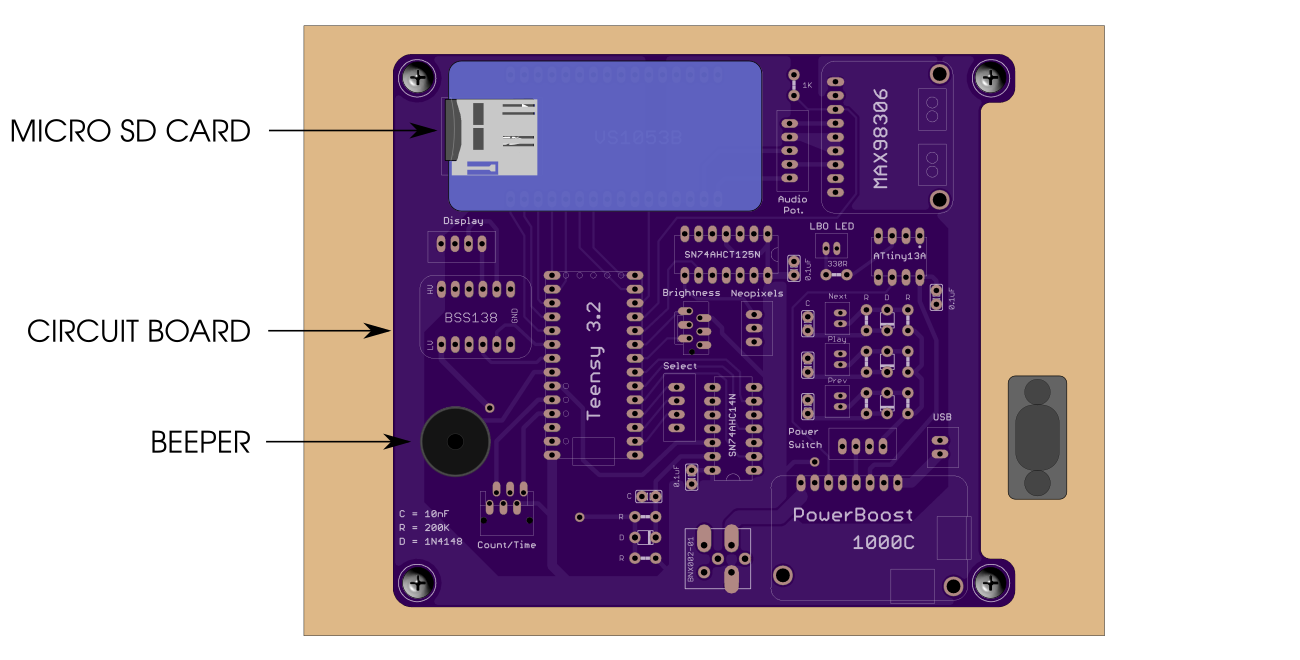
\includegraphics{images/back_circuit_board.png}
\caption{Back - Circuit Board}
\end{figure}

%%%%%%%%%%%%%%%%%%%%%%%%%%%%%%%%%%%%%%%%%%%%%%%%%%%%%%%%%%%%%%%%%%%%%%%%%%%%%%%%
% Back - Power / Charge Port
%%%%%%%%%%%%%%%%%%%%%%%%%%%%%%%%%%%%%%%%%%%%%%%%%%%%%%%%%%%%%%%%%%%%%%%%%%%%%%%%
\section{Power / Charge Port} \label{Power Port}

The \cPP{f} is a \cUSB{f} port.

\par\medskip

A few items of note:

\begin{itemize}
  \item The device can be \sON{f} or \sOFF{f} when plugging or unplugging the
    \hyperref[Power Adapter]{\cPA{f}} or other USB cable.
  \item The device can be \sON{f} or \sOFF{f} while charging.
  \item The device is fully functional while charging.
  \item The device never has to be unplugged.\footnote{ It should be unplugged
    when \hyperref[Cleaning]{cleaning} and
    \hyperref[Disassembly]{disassembling}.}
\end{itemize}

See \hyperref[Powering and Recharging]{Powering \& Recharging} for more
information.

%%%%%%%%%%%%%%%%%%%%%%%%%%%%%%%%%%%%%%%%%%%%%%%%%%%%%%%%%%%%%%%%%%%%%%%%%%%%%%%%
% Back - Beeper
%%%%%%%%%%%%%%%%%%%%%%%%%%%%%%%%%%%%%%%%%%%%%%%%%%%%%%%%%%%%%%%%%%%%%%%%%%%%%%%%
\section{Beeper} \label{Beeper}

The \cBe{f} is a \mono{2.3\thinspace kHz} magnetic single tone buzzer and is
used with the \hyperref[Alarm]{\mAl{f}}, \hyperref[Timer]{\mTi{f}} and
\hyperref[Touch Settings]{\mTS{f}}.  Note, it will always sound at the same
volume since the \cVo{f} control is not connected to it and can \textit{not}
adjust it.

\par\medskip

There are two symbols used to reference the \cBe{f} that are used in later
sections.

\begin{table}[H]
\ers{2}
\centering
\begin{tabu}{X[1,c,m] | X[5,l,m]}
  \thrule
  \thbi{Symbol} & \thbi{Meaning} \\ \mrule
  \sBe & The \cBe{f} is making sound, i.e. beeping. \\ \drule{2}
  \sNBe & The \cBe{f} is mute, i.e. \textit{not} beeping. \\
  \bhrule
\end{tabu}
\end{table}

%%%%%%%%%%%%%%%%%%%%%%%%%%%%%%%%%%%%%%%%%%%%%%%%%%%%%%%%%%%%%%%%%%%%%%%%%%%%%%%%
% Back - Micro SD Card
%%%%%%%%%%%%%%%%%%%%%%%%%%%%%%%%%%%%%%%%%%%%%%%%%%%%%%%%%%%%%%%%%%%%%%%%%%%%%%%%
\section{Micro SD Card} \label{Micro SD Card}

The \cMSD{f} is used as storage for the songs on the device.  The \cMSD{f} that
comes preinstalled with the device has a read speed of at least
\num{90} \mono{MB/sec} and is formatted with the \mono{FAT32} filesystem using
\num{512} bytes per sector.

%%%%%%%%%%%%%%%%%%%%%%%%%%%%%%%%%%%%%%%%%%%%%%%%%%%%%%%%%%%%%%%%%%%%%%%%%%%%%%%%
% Accessories
%%%%%%%%%%%%%%%%%%%%%%%%%%%%%%%%%%%%%%%%%%%%%%%%%%%%%%%%%%%%%%%%%%%%%%%%%%%%%%%%
\chapter{Accessories} \label{Accessories}

%%%%%%%%%%%%%%%%%%%%%%%%%%%%%%%%%%%%%%%%%%%%%%%%%%%%%%%%%%%%%%%%%%%%%%%%%%%%%%%%
% Accessories - Hex Driver
%%%%%%%%%%%%%%%%%%%%%%%%%%%%%%%%%%%%%%%%%%%%%%%%%%%%%%%%%%%%%%%%%%%%%%%%%%%%%%%%
\section{Hex Driver} \label{Hex Driver}

A \mono{3/32"} hex driver is included for the purpose of removing and replacing
the \hyperref[Fastening Screws]{Fastening Screws} that hold the enclosure
together.

\begin{figure}[H]
\centering
  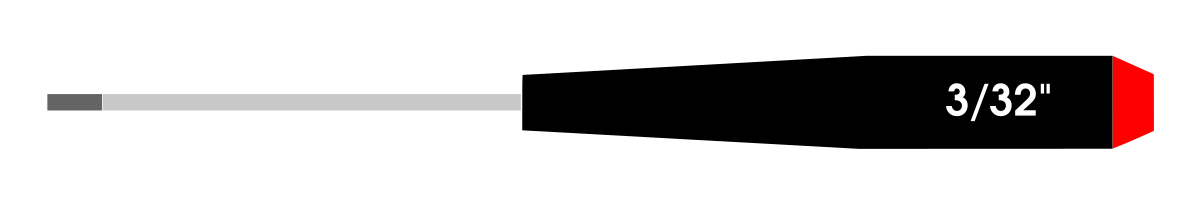
\includegraphics{images/hex_driver.png}
\caption{3/32" Hex Driver}
\end{figure}

\warning{Before taking the enclosure apart, please refer to
\hyperref[Disassembly]{Disassembly}.}

%%%%%%%%%%%%%%%%%%%%%%%%%%%%%%%%%%%%%%%%%%%%%%%%%%%%%%%%%%%%%%%%%%%%%%%%%%%%%%%%
% Accessories - Power Adapter
%%%%%%%%%%%%%%%%%%%%%%%%%%%%%%%%%%%%%%%%%%%%%%%%%%%%%%%%%%%%%%%%%%%%%%%%%%%%%%%%
\section{Power Adapter} \label{Power Adapter}

The \cPA{f} is used to both power the device
and charge the \hyperref[Rechargeable Battery]{\cRB{f}}.  It is a
\mono{5.25\thinspace V}, \mono{2.4\thinspace A} switching AC/DC power adapter
that terminates with a \cUSB{f} connector that plugs into the
\hyperref[Power Port]{\cPP{f}}.  It can accept either \num{110} or \num{240}
\mono{VAC} mains so works in the US as well as other countries.

\par\medskip

If this needs to be replaced, the replacement \textit{must} be a
\mono{5\thinspace V} AC/DC adapter (or \mono{5.25\thinspace V} if you can find
one).

\danger{An adapter that is \mono{6\thinspace V}, \mono{9\thinspace V},
\mono{12\thinspace V} or above \textit{will} damage the device.}

\warning{An adapter that is less than \mono{5\thinspace V} will not be able to
power the device and it \textit{will} malfunction.}

The adapter should be rated for at least \mono{1\thinspace A} and no more than
\mono{2.5\thinspace A}.

%%%%%%%%%%%%%%%%%%%%%%%%%%%%%%%%%%%%%%%%%%%%%%%%%%%%%%%%%%%%%%%%%%%%%%%%%%%%%%%%
% Powering & Recharging
%%%%%%%%%%%%%%%%%%%%%%%%%%%%%%%%%%%%%%%%%%%%%%%%%%%%%%%%%%%%%%%%%%%%%%%%%%%%%%%%
\chapter{Powering \& Recharging} \label{Powering and Recharging}

The device can be both powered and charged using either the supplied
\hyperref[Power Adapter]{\cPA{f}} or a \textit{USB 2.0 Standard Type-A Male to
Micro Type-B Male} cable.

\par\medskip

\cUSB{f} is asymmetric and can only be plugged in one way.

\begin{figure}[H]
\centering
  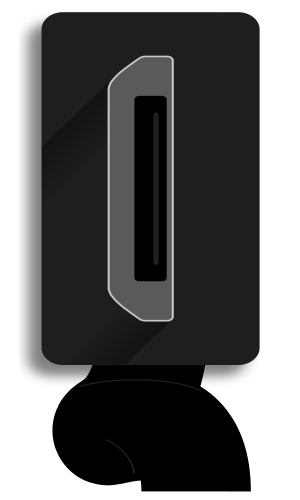
\includegraphics{images/usb.png}
\caption{USB 2.0 Micro-B}
\end{figure}

The figure below indicates how the USB 2.0 Micro-B plug should be oriented when
\textit{facing} the \hyperref[Power Port]{\cPP{f}}.

\begin{figure}[H]
\centering
  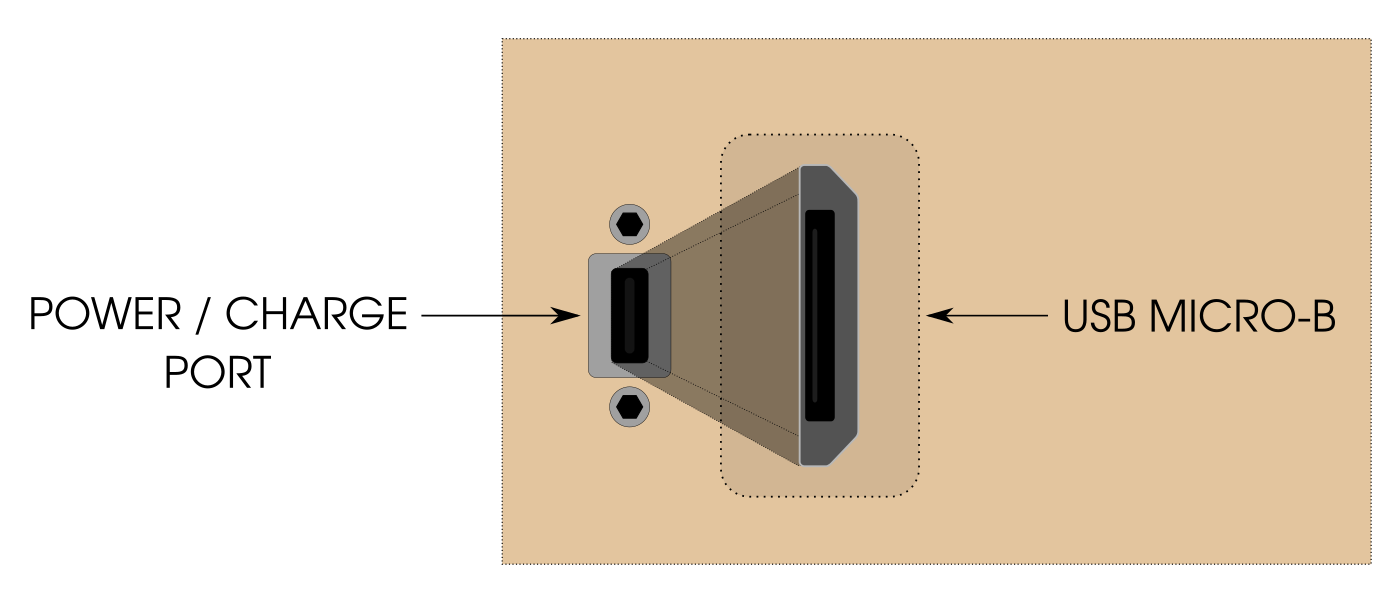
\includegraphics{images/usb_orientation.png}
\caption{USB 2.0 Micro-B $\longrightarrow$ Power / Charge Port Orientation}
\end{figure}

Using the supplied \cPA{f}, plug the \cUSB{f} end into the \cPP{f} on the
\cBa{f} of the device and the 2-prong end into a wall or power strip receptacle.

\par\medskip

If a \textit{USB 2.0 Standard Type-A Male to Micro Type-B Male} cable is used,
connect the Micro-B end into the \cPP{f} and the Standard Type-A end into the
USB port on a computer or USB hub.

%%%%%%%%%%%%%%%%%%%%%%%%%%%%%%%%%%%%%%%%%%%%%%%%%%%%%%%%%%%%%%%%%%%%%%%%%%%%%%%%
% Powering & Recharging - Recharging
%%%%%%%%%%%%%%%%%%%%%%%%%%%%%%%%%%%%%%%%%%%%%%%%%%%%%%%%%%%%%%%%%%%%%%%%%%%%%%%%
\section{Recharging} \label{Recharging}

The \hyperref[Low Battery Indicator]{\cLB{f}} will light up when the device
needs to be recharged.  Unfortunately there is no way to indicate that the
battery has finished charging. Using the supplied
\hyperref[Power Adapter]{\cPA{f}}, it should take about \num{8} hours to charge
if the \cLB{f} is signaling - plug it in before going to bed and it should be
charged by the time you wake up.  When using a \textit{USB 2.0 Standard Type-A
Male to Micro Type-B Male} cable, charging may take longer since USB ports on a
computer generally do not supply as much current as the \cPA{f} will.

